% Chapter Template

\chapter{Methodology}

\label{Methodology}

\section{Pose}

The methodology throughout this section is dependent on pose information output from models that were described in section \ref{sec:pose-detection}. These pose models output several outputs used by similar models such as joint heatmaps, however the main focus of this paper is the pure positions of the joints. These joints can be connected by lines to form "bones" which are then all connected together to form a "skeleton". This skeleton is shown in figure \ref{fig:pose}, where each of the joints are connected to form a human-like figure that can easily be created form the x \& y coordinates of the joints.

\begin{figure}[ht]
	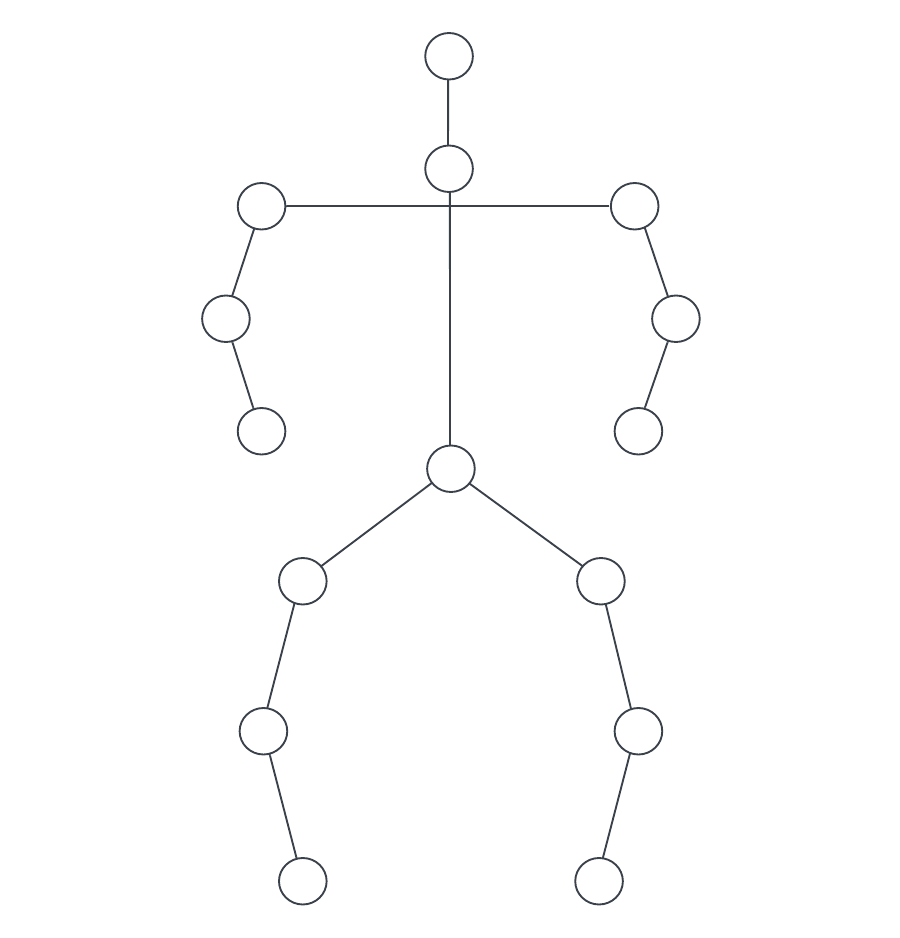
\includegraphics[width=5cm]{pose}
	\centering
	\caption{Example of how joints are connected through bones in pose representations.}
	\label{fig:pose}
\end{figure}

Using the JHMDB dataset, we simply take the existing pose implementation, the representation and indexes being shown in figure \ref{fig:JHMDB}, where there are 15 total joints. Specifically in this thesis, we are concerned with bone-joint-bone connections, effectively representing the angle of the middle joint and how the bones around it move.

\subsection{Joint Angles}

The core of how the new representation will represent actions and movement have to do with the angle between two bones at any one given joint.

\begin{figure}[ht]
	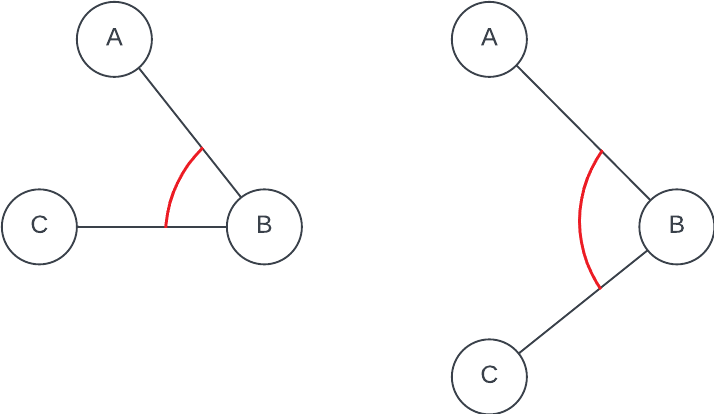
\includegraphics[width=5cm]{JointAngles}
	\centering
	\caption{}
	\label{fig:joint-angles}
\end{figure}

The first step in calculating the directional angle between the two vectors is to center them at the origin. Throughout this chapter, we will be referring to these two vectors as $a$ and $b$. Which in figure \ref{fig:joint-angles}, "$a$" would be denoting the vector $B \rightarrow A$ and "$b$" the vector $B \rightarrow C$. This origin centering is simple and is done by the following equation \ref{eqn:angle-centering}, with each point representation as it was in figure \ref{fig:joint-angles} using the $B \rightarrow A$ bone as an example.

\begin{equation}
	\label{eqn:angle-centering}
	\centering
	VectorA(x,y) = (A.x - B.x, A.y - B.y)
\end{equation}

After processing both bones through this equation, it produces two vectors beginning at the origin. The goal then becomes calculating the angle between two of these vectors. This can be easily done by leveraging arctan. Calculating the angle of a given vector '$a$' to the x-axis is simply done by using $\arctan(a.y/a.x)$. Once we have the angle of this vector to the x-axis, we can convert it to a positive value to ensure that the angle is being measured from a clockwise direction. Afterwards, we simply take the difference of the two vectors to determine the clockwise directional angle between two given vectors as denoted in equation \ref{eqn:angle-calculation}.

\begin{equation}
	\label{eqn:angle-calculation}
	\centering
	\arctan(a.y/a.x) - \arctan(b.y/b.x)
\end{equation}

The angle is calculated in a particular direction because if it were simply to be calculated agnostic of direction, it would be impossible to determine what angle a joint moves if it were to cross the $180^\circ$ boundary. Table \ref{tab:directed-angle-example} demonstrates this issue, where a $180^\circ$ rotation is observed from one right angle to another, but if non-directional angle is used, no change is represented.

\begin{table}[ht]
	\centering
	\begin{tabular}{||c c c c||} 
		\hline
		\textbf{a(x,y)} & \textbf{b(x,y)} & \textbf{Directional Diff} & \textbf{Non-Directional Diff} \\ [0.5ex] 
		\hline\hline
		$(1,0)$ & $(0,1)$ & $90^\circ$ & $90^\circ$ \\
		\hline
		$(1,0)$ & $(0,-1)$ & $270^\circ$ & $90^\circ$ \\
		\hline
	\end{tabular}
	\caption{Example of how non-directional angle can result in incorrect rotation changes from one frame to another.}
	\label{tab:directed-angle-example}
\end{table}

The resulting method means that some angles will be measured from the "outside" of the person and some will be measured from the "inside" as shown in figure \ref{fig:pose-joint-angles}. In practice, this does not have a large effect on the representation as the primary factor in this method is the change of an angle from one frame to another which is indifferent to how the angle is measured as long as the distance is consistent.

\begin{figure}[ht]
	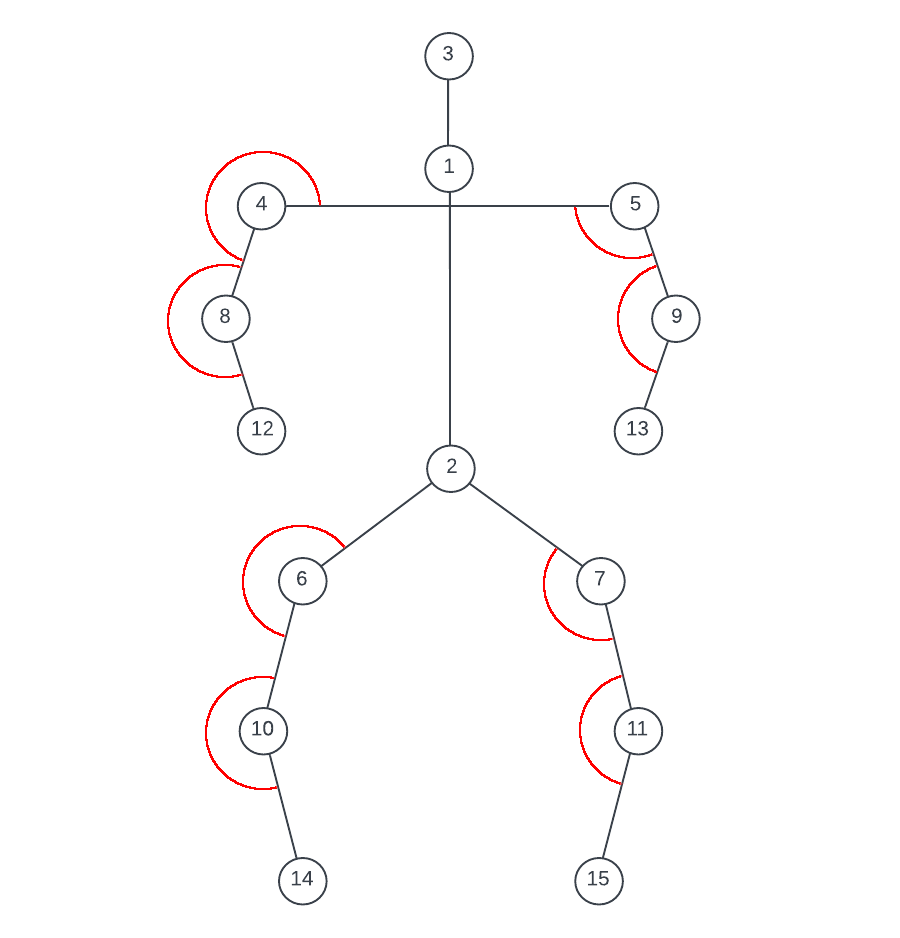
\includegraphics[width=5cm]{PoseJointAngles}
	\centering
	\caption{}
	\label{fig:pose-joint-angles}
\end{figure}

\subsection{Joint Velocities}
\label{sec:joint-velocities}

Once the joint angles for each frame have been extracted, the next step before implementation into our representation is to determine the change of a joint angle from one frame to another to determine the "velocity" of said joint angle. Generally this is simply done by calculating $angle(b) - angle(a)$, however there is one exception where the angle change crosses over the positive x-axis. This would be an example such as the difference between $a = 5$ and $b = 350$. The correct description would be that the angle moved $-15^\circ$, however using that simple calculation would mean that the model would interpret this as a $345^\circ$ change. This is most likely incorrect, as the more likely scenario is that the person moved $-15^\circ$ rather than almost a complete rotation in the other direction. So we add logic such that if the difference between two angles is greater than $180^\circ$ or lower than $-180^\circ$, the most likely scenario is that it moved in the opposite direction for a shorter distance. So a change such as $270^\circ$ would become $-90^\circ$ and similarly a change of $-270^\circ$ would become $90^\circ$.

\section{Novel Intermediate Representation}

Using this logic, we can now construct the indermediate representation that will be used as input to our model. The model representation is very similar to that in the \textbf{Simple yet efficient real-time pose-based action recognition} \cite{simple_yet_efficient} as described in section \ref{sec:intermediate}, which involves constructing a 2 dimensional image that is easily fed into a simple model. This is represented in figure \ref{fig:intermediate-construction}, where one joint angle is taken from one frame of the video, and added to a column. This column consists of all of the data for one frame of the video, which is then added to the rest of the representation, eventually constructing the joint angles for each frame of the video.

\begin{figure}[ht]
	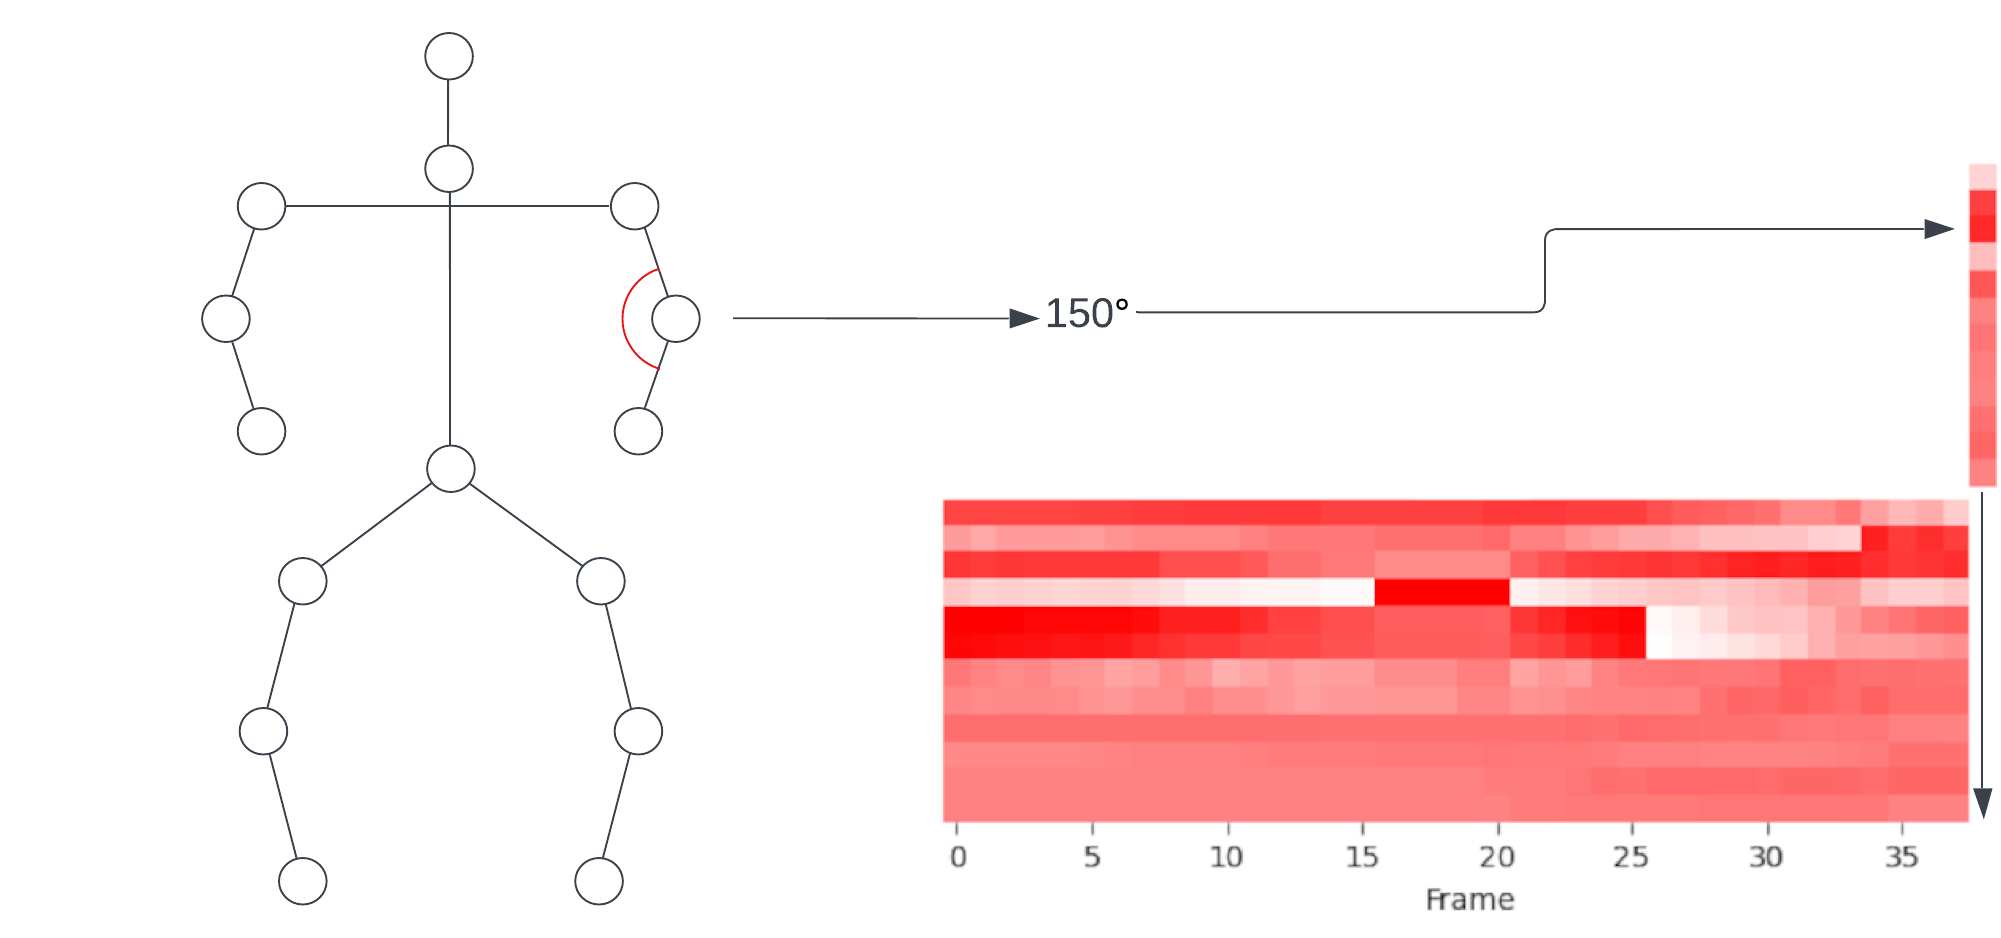
\includegraphics[width=8cm]{IntermediateConstruction}
	\centering
	\caption{}
	\label{fig:intermediate-construction}
\end{figure}

As described previously in section \ref{sec:joint-velocities}, a key point of our representation is the joint velocities portion. These values can simply be "stacked" on top of the angles to form the full intermediate representation. The logic is that for any given frame $i$, the column contains both the joint angles for the frame $i$, as well as their differences between frame $i$ \& $i+1$.

\begin{figure}[ht]
	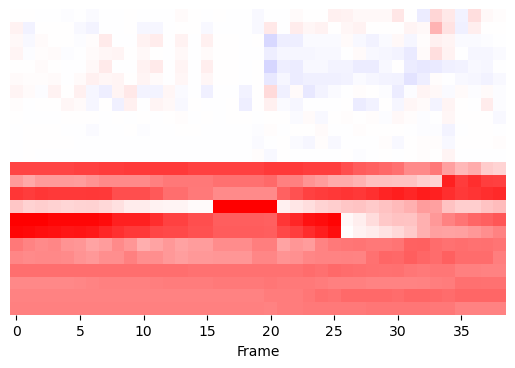
\includegraphics[width=8cm]{IntermediateStacked}
	\centering
	\caption{}
	\label{fig:intermediate-stacked}
\end{figure}

The specific joints that are represented in our intermediate representation are shown in table \ref{tab:joint-connections}. These joints were chosen as they are major joints that form the typical "skeleton" visualization similar to that shown in figure \ref{fig:pose} or figure \ref{fig:pose-joint-angles}.

\begin{table}[ht]
	\centering
	\begin{tabular}{||c c c c||} 
		\hline
		\textbf{Joint A} & \textbf{Joint B} & \textbf{Joint C} & \textbf{JHMDB Indices} \\ [0.5ex] 
		\hline\hline
		Face & Neck & Right Shoulder & $(3, 1, 4)$ \\
		Face & Neck & Left Shoulder & $(3, 1, 4)$ \\
		\hline
		Right Elbow & Right Shoulder & Left Shoulder & $(8, 4, 5)$ \\
		Left Elbow & Left Shoulder & Right Shoulder & $(9, 5, 4)$ \\
		\hline
		Right Elbow & Right Shoulder & Right Hip & $(8, 4, 6)$ \\
		Left Elbow & Left Shoulder & Left Hip & $(9, 5, 7)$ \\
		\hline
		Right Wrist & Right Elbow & Right Shoulder & $(12, 8, 4)$ \\
		Left Wrist & Left Elbow & Left Shoulder & $(13, 9, 5)$ \\
		\hline
		Right Shoulder & Right Hip & Right Knee & $(4, 6, 10)$ \\
		Left Shoulder & Left Hip & Left Knee & $(5, 7, 11)$ \\
		\hline
		Right Hip & Right Knee & Right Ankle & $(6, 10, 14)$ \\
		Left Hip & Left Knee & Left Ankle & $(7, 11, 15)$ \\
		\hline
	\end{tabular}
	\caption{All Joint connections used in our intermediate representations.}
	\label{tab:joint-connections}
\end{table}

\subsection{Temporal Adjustments}

It is not unreasonable to assume that moving from only one frame to the next would result in some actions not being represented as well as other actions. Due to this issue, we add a temporal adjustment to our representation in order to better represent some of these actions. This is done by adding more channels to the data, with each of the channels "skipping" frames. This would mean that rather than having the angle difference representation moving from frames $1 \rightarrow 2 \rightarrow 3$, in the first additional channel it would move from frames $1 \rightarrow 3 \rightarrow 5$. The representation is then padded out to fi the same shape and added as another channel to the data. This is more clearly shown in figure \ref{fig:intermediate-stacked-skip} where the actions become more "compressed" and movements over longer periods of time become easier to visualize and process.

\begin{figure}[ht]
	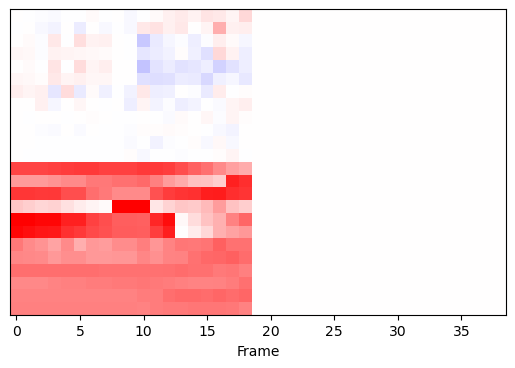
\includegraphics[width=8cm]{IntermediateSkip1}
	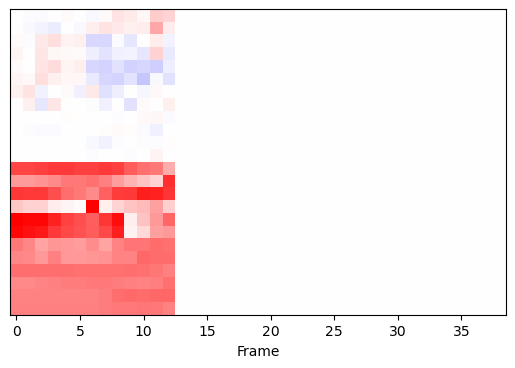
\includegraphics[width=8cm]{IntermediateSkip2}
	\centering
	\caption{}
	\label{fig:intermediate-stacked-skip}
\end{figure}

\subsection{Model Architecture}

\begin{figure}[ht]
	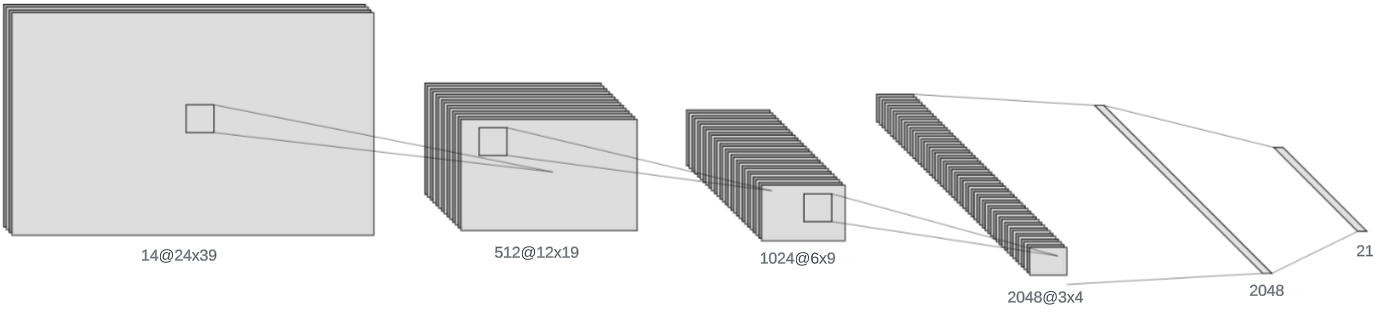
\includegraphics[width=12cm]{ModelArchitecture}
	\centering
	\caption{}
	\label{fig:model-architecture}
\end{figure}

The goal of this intermediate representation is to be able to use a simple 2-dimensional CNN which is able to run on simpler and less expensive hardware. The simplified architecture diagram in figure \ref{fig:model-architecture} shows the simple CNN architecture that is to be used. The model consists of 3 convolutional layer groups, followed by global average pooling and the final classification layer. Each individual layer and a more detailed breakdown is shown in table \ref{tab:detailed-model}.

\begin{table}[ht]
	\centering
	\begin{tabular}{||c||}
		\hline
		2D Convolution @ 512 Channels \\
		2D Batch Normalization \\
		ReLU \\
		2D Convolution @ 512 Channels \\
		2D Batch Normalization \\
		ReLU \\
		2D Max Pooling\\
		\hline\hline
		50\% Dropout \\
		2D Convolution @ 1024 Channels \\
		2D Batch Normalization \\
		ReLU \\
		2D Convolution @ 1024 Channels \\
		2D Batch Normalization \\
		ReLU \\
		2D Max Pooling\\
		\hline\hline
		50\% Dropout \\
		2D Convolution @ 2048 Channels \\
		2D Batch Normalization \\
		ReLU \\
		2D Convolution @ 2048 Channels \\
		2D Batch Normalization \\
		ReLU \\
		2D Max Pooling\\
		\hline\hline
		Global Average Pooling \\
		Flatten \\
		21 Class Softmax Layer \\
		\hline
	\end{tabular}
	\caption{The detailed breakdown of the model architecture, split into 3 convolutional blocks and one dense layer used for classification. All convolutional layers utilize 3x3 convolutions, including a 1 pixel padding across all sides. The 2D max pooling utilized a 2x2 kernel, halving the size of the images after each convolutional block.}
	\label{tab:detailed-model}
\end{table}